\chapter{Optimal Level of Labor Supply}
\label{ch:optimum}
\thispagestyle{fancy}

In our model, any participant of the labor market can decide at any point in time, whether or not she wants to supply an extra unit of labor. She is therefore confronted with a budget line like the one shown in figure \ref{graph:budgetline} in blue. According to the neoclassical model of labor-leisure choice (NLC) she chooses her supplied work so as to achieve the highest possible indifference curve $\text{U}^*$.\\

\begin{figure}[ht!]
    \centering
    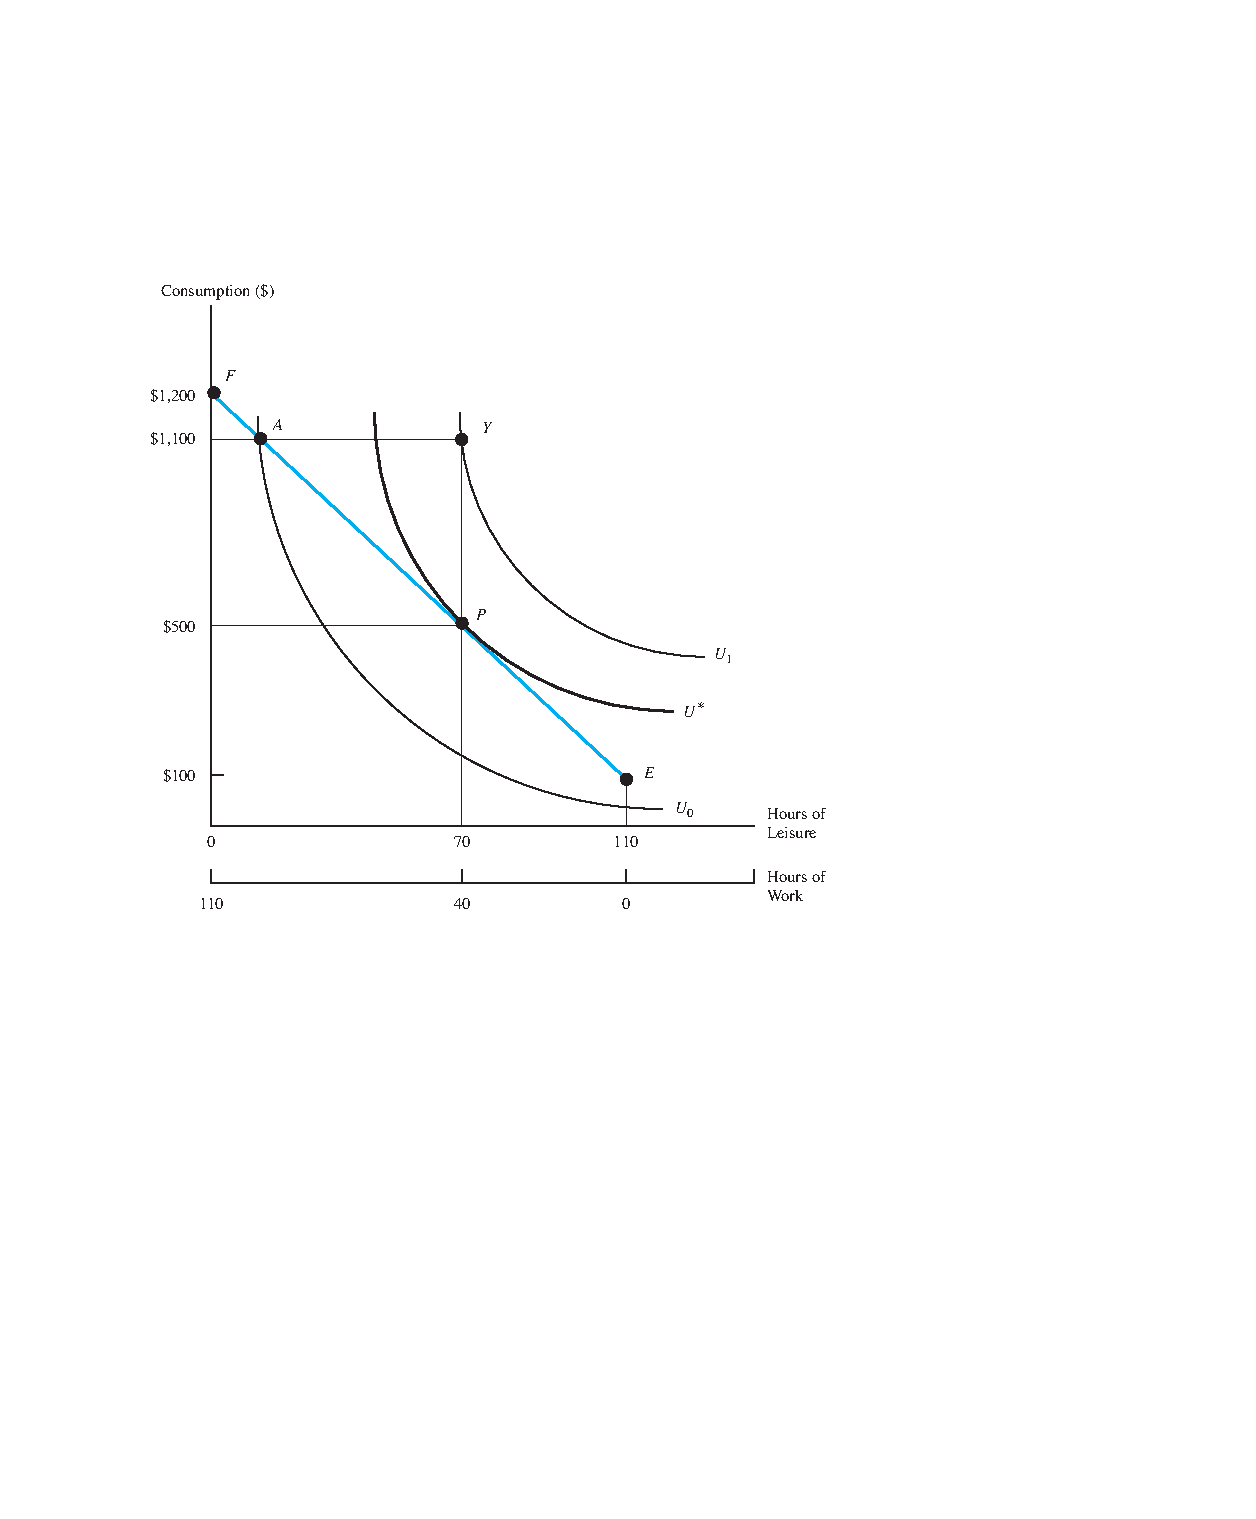
\includegraphics[scale = 0.60]{graphs/budget_line.pdf}
    \caption{The Neoclassical Model of Labor-Leisure Choice (\cite{borjas2012})}
    \label{graph:budgetline}
\end{figure}

When we introduce a fixed benefit as in the UBI, we increase the initial endowment of each citizen and so move the budget line parallel upwards as shown in figure \ref{graph:budgetline2}. It is fair to assume that leisure is a normal good and that, all other elements kept constant, people will choose more of it if they earn more. NLC predicts therefore an unambiguous negative shift in labor supplied (\cite{borjas2012}).\\

\begin{figure}[ht!]
    \centering
    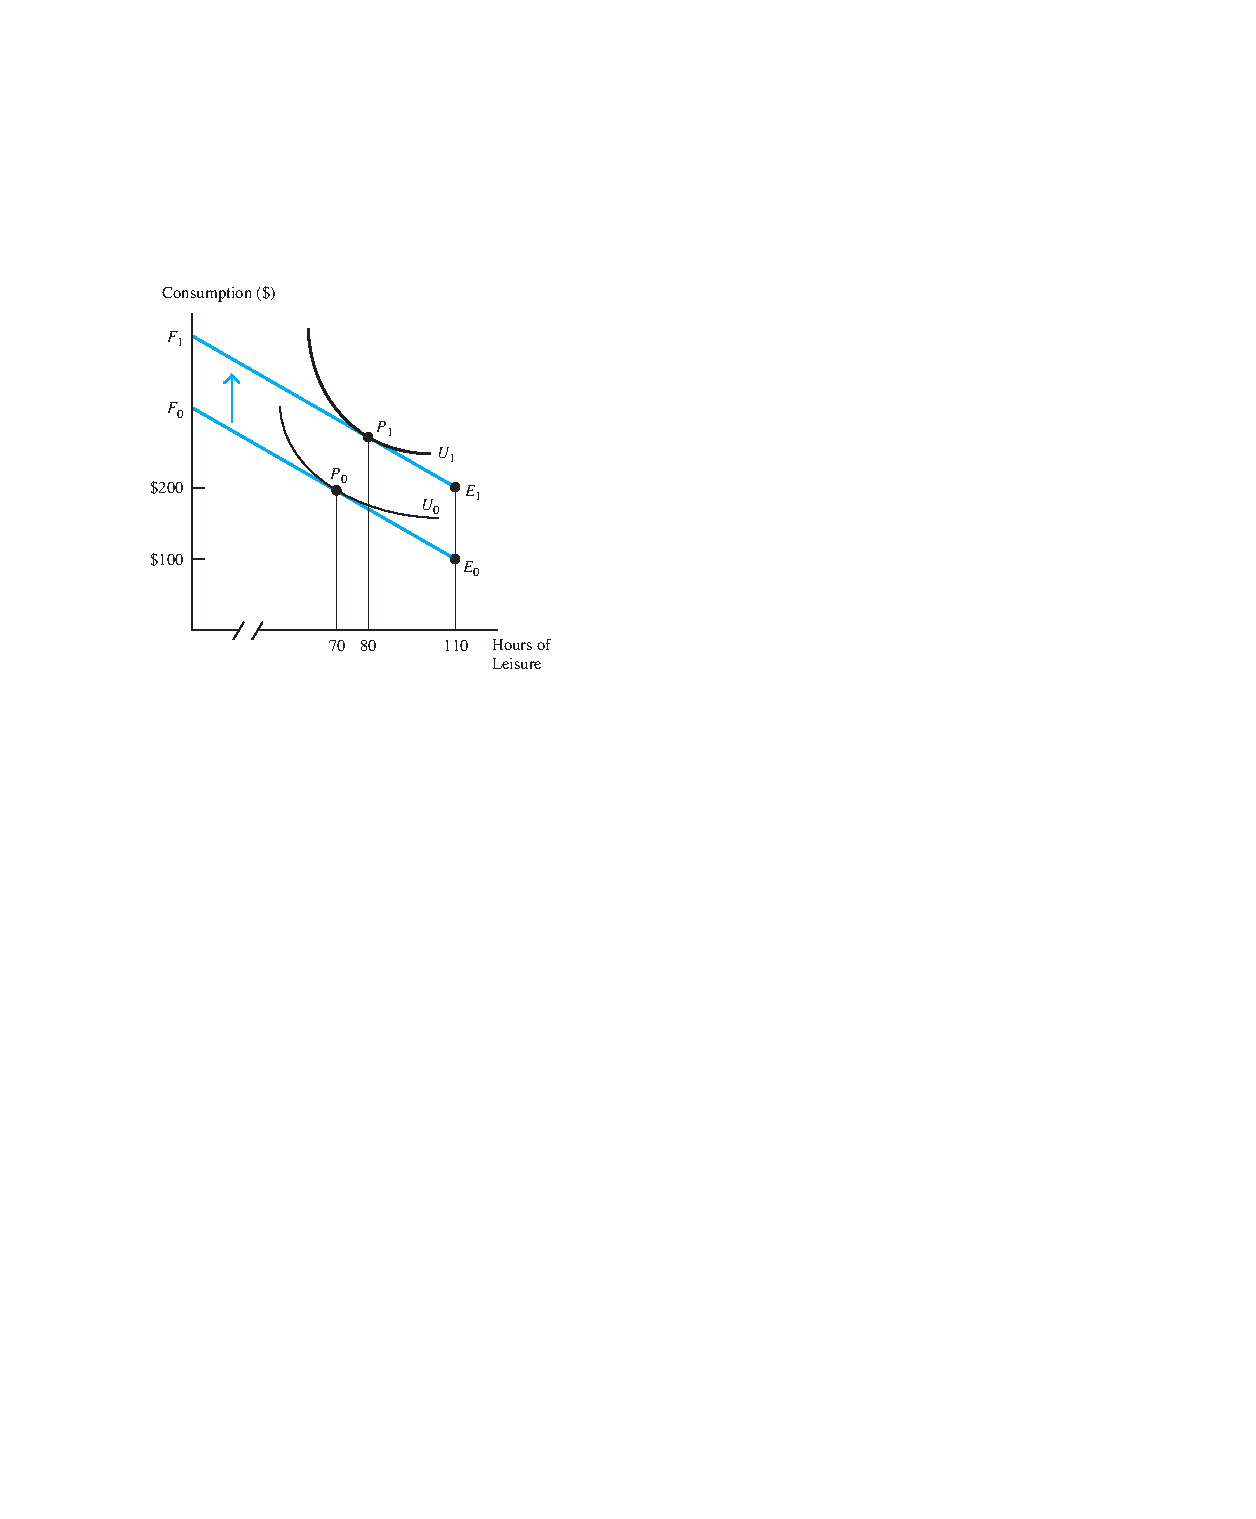
\includegraphics{graphs/budget_line_2.pdf}
    \caption{A parallel upward movement of the Budget Line (\cite{borjas2012})}
    \label{graph:budgetline2}
\end{figure}


Subsequently, after the introduction of a taxation scheme, the budget line of a citizen pivots around their initial endowment as shown in figure \ref{graph:price_change}. Given the same amount of work supplied, she can now consume less goods. Her reaction to this relative change in prices in terms of work supplied is the combination of two effects. On the one hand, she can now afford less and would like to work more: an income effect. On the other hand, the opportunity cost of leisure is reduced what incentivises her to work less: a substitution effect. Figure \ref{graph:price_change} illustrates this phenomena.\\

The Slutsky Equation (eq. \ref{eq:slutsky}) shows in a general form the impact of both the substitution and the income effect on the total effect of labor supply. It is obtained by total-derivating the Hicksian and Marshallian duality equation (a proof is presented in the Appendix). The first term on the right represents the substitution effect while the second represents the income effect. The negative sign of the income effect signalises, that given a positive change in wage, labor supply is reduced while the substitution effect increases labor supply. The direction of change in labor supply after the introduction of an NIT will depend on whether the substitution or the income effect dominates for each individual (\cite{varian1992}). Note that while we cannot directly observe utility and therefore the substitution effect, we can estimate it from the changes in the other two terms. \\

\begin{equation}
  \underbrace{\frac{\partial x_i (\mathbf{p},w)}{\partial p_j}}_{\text{Total Effect}}
=\underbrace{\frac{\partial h_i (\mathbf{p},\bar u)}{\partial p_j}}_{\text{Substitution Effect}}
-\underbrace{\frac{\partial x_i (\mathbf{p}, w)}{\partial w}
x_j(\mathbf{p},w)}_{\text{Income Effect}}
\label{eq:slutsky}
\end{equation}

\begin{figure}[H]
    
    \begin{subfigure}{0.5\textwidth}
    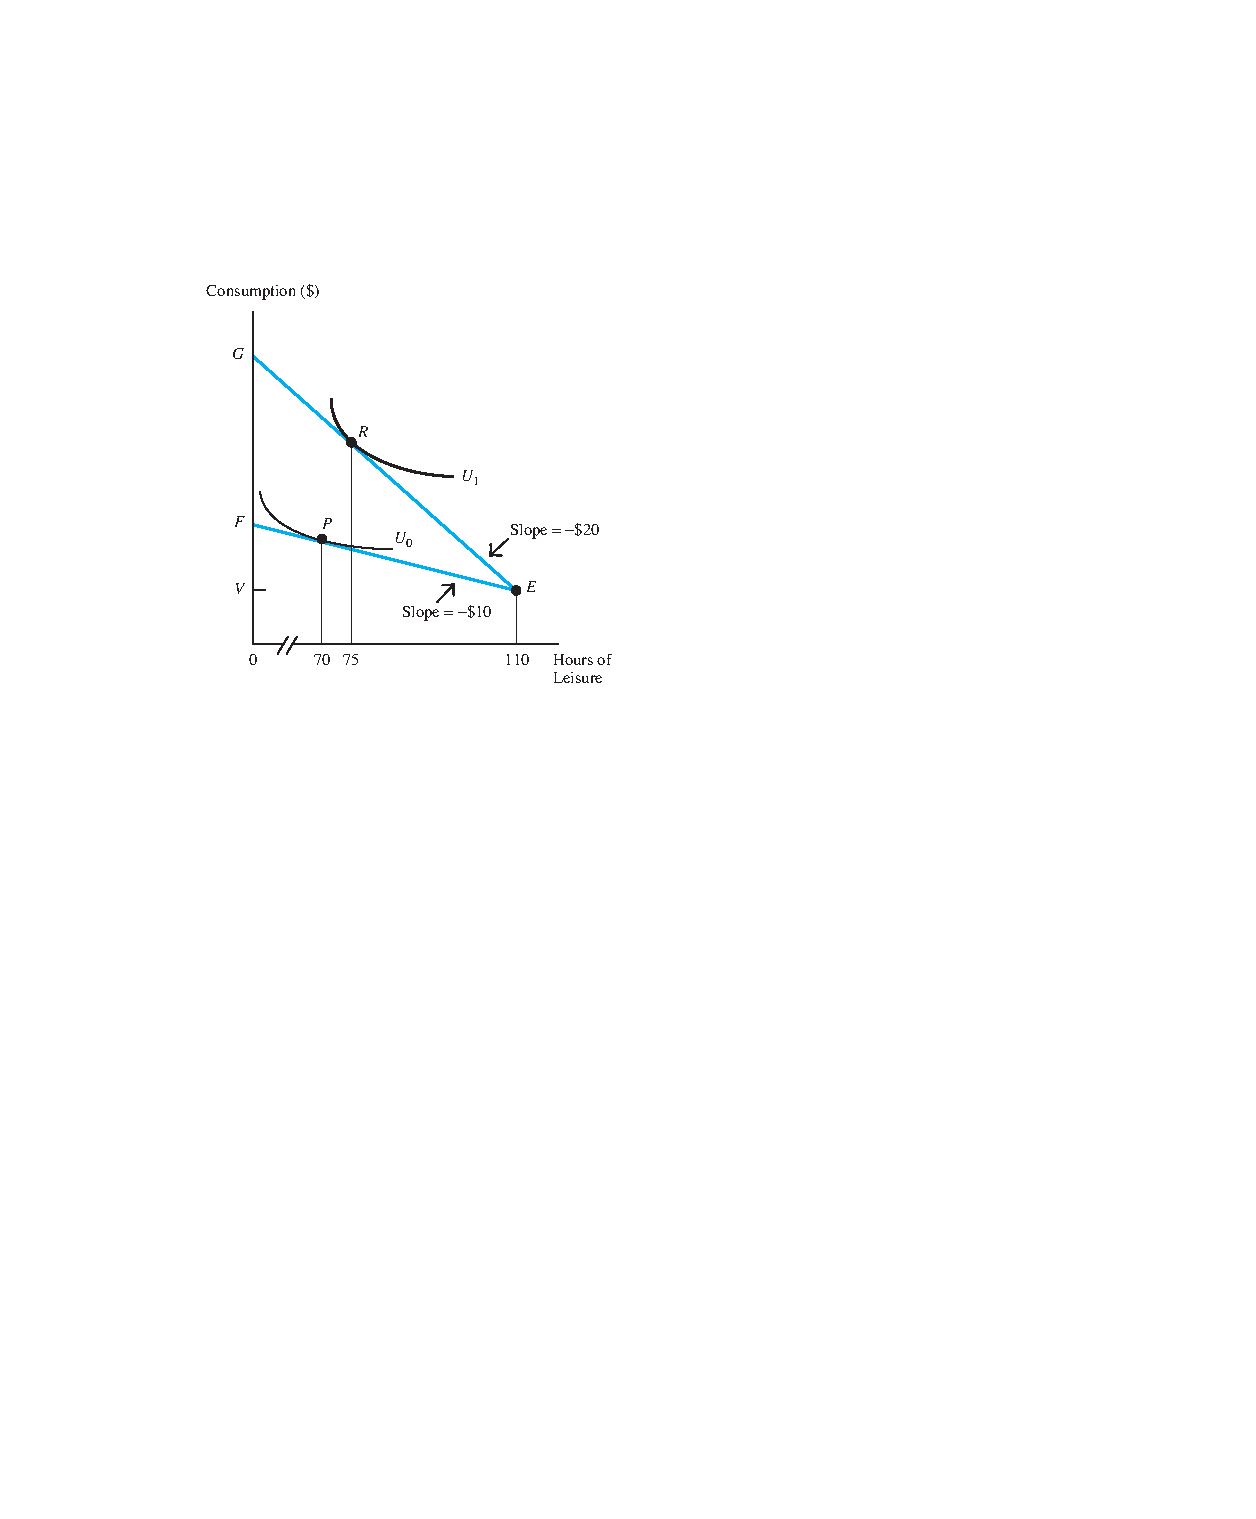
\includegraphics[scale = 0.75]{graphs/budget_line_3-1.pdf}
    \caption{Income Effect Dominates}
    \label{graph:budgetline31}
    \end{subfigure}
    \begin{subfigure}{0.5\textwidth}
    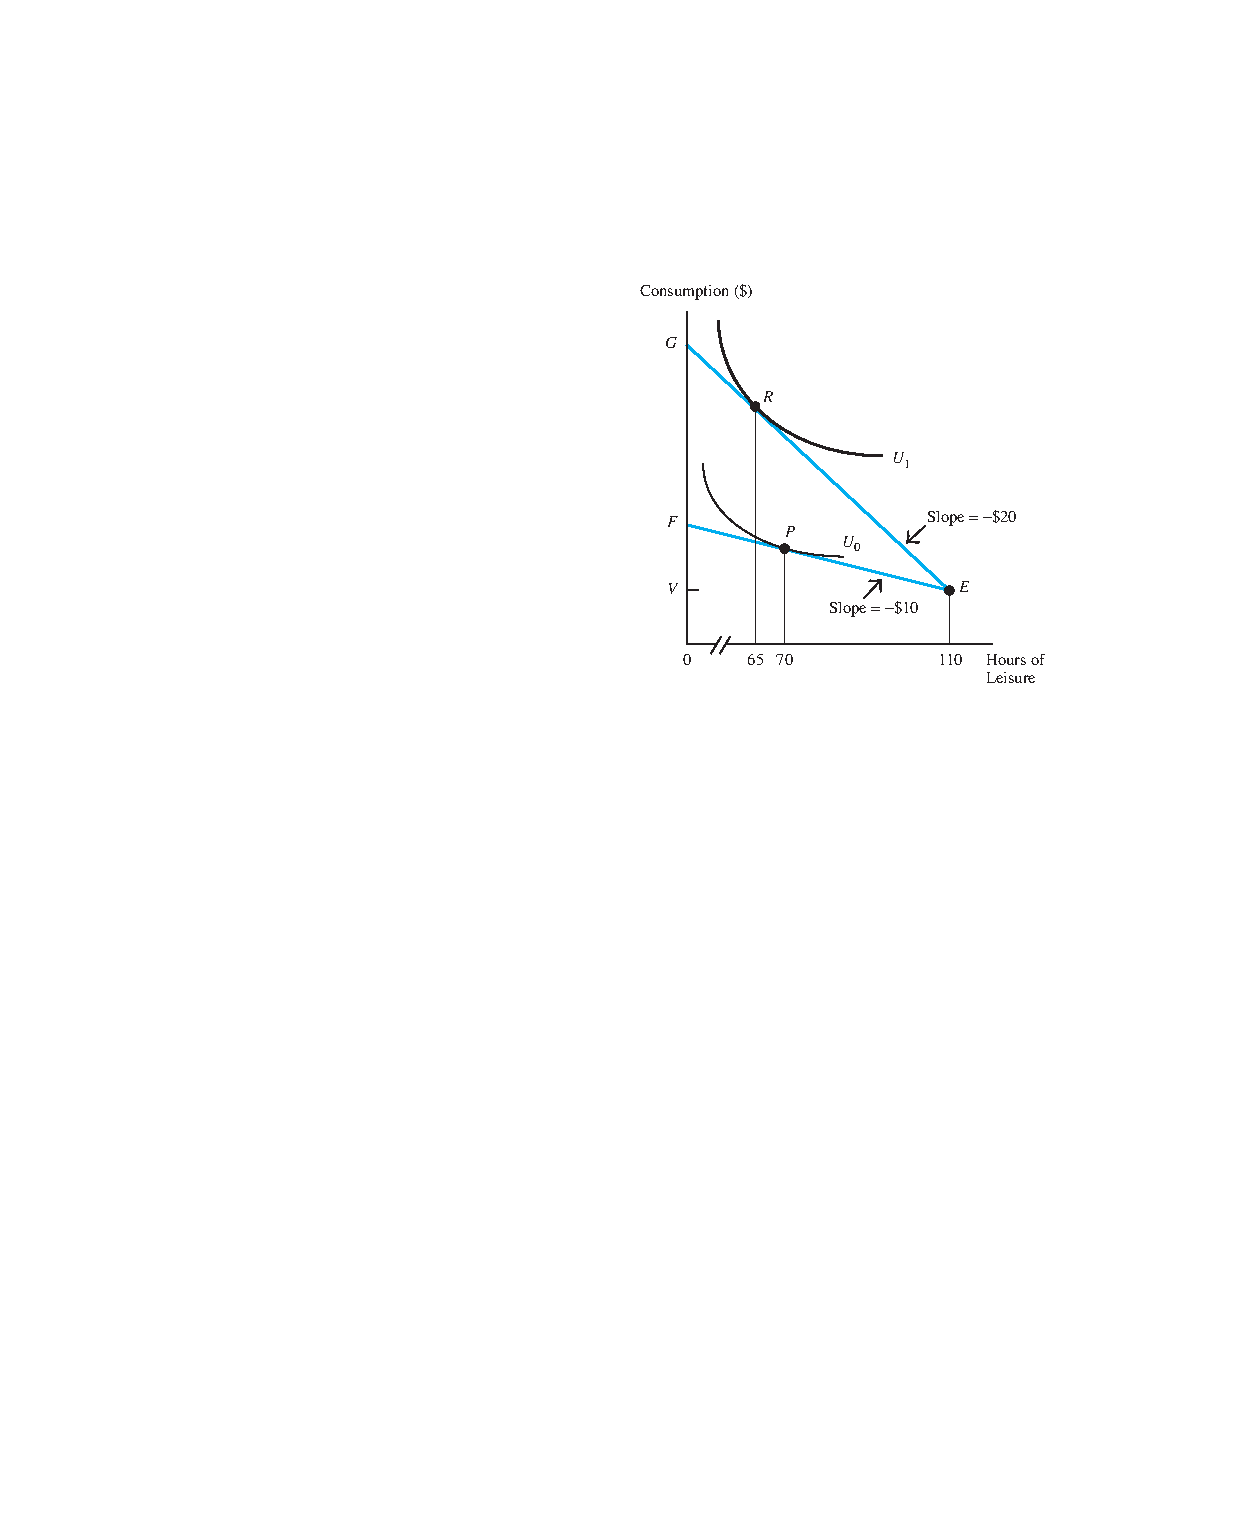
\includegraphics[scale = 0.75]{graphs/budget_line_3-2.pdf}
    \caption{Substitution Effect Dominates}
    \label{graph:budgetline32}
    \end{subfigure}
\caption{Change in the Relative Price of Leisure (\cite{borjas2012})}
\label{graph:price_change}
\end{figure}

After introducing a tax-and-benefit system like the NIT or the UBI, depending on their status as net-payers or net-receivers, citizens will be confronted with a different change in their budget constraints. While a citizen below threshold $k$ earns more for any given amount of work supplied, a citizen above $k$ will receive less. Assuming that in the aggregate either a substitution or an income effects dominates, we should observe a different trend in labor supply for the group under and above the taxation threshold.\\ 

Although in the model developed in section \ref{ch:experiment} the UBI and the NIT are equivalent, it is important to note that, at first, the change into an UBI looks to a participant like an increase of non-labor income without relative price changes. The introduction of an NIT, on the contrary, is immediately equal to both an increase in non-labor income and a change in relative prices. Participants might therefore decide on their labor supply differently between both systems and in the former case reduce the supplied labor across the board.

